% !TeX spellcheck = ru_RU
\section{Протокол TCP}
\subsection{Заголовок TCP}
\begin{table}[h]
	\begin{tabular}{|c|c|c|c|c|c|c|}
		\hline
		Бит & 0-3 & 4-9 & 10-15 & \multicolumn{3}{c|}{16-31} \\ \hline
		0   & \multicolumn{3}{c|}{\begin{tabular}[c]{@{}c@{}}Source Port\\ порт отправителя\end{tabular}}                                                                                                          & \multicolumn{3}{c|}{\begin{tabular}[c]{@{}c@{}}Destination Port\\ порт получателя\end{tabular}}  \\ \hline
		32  & \multicolumn{6}{c|}{\begin{tabular}[c]{@{}c@{}}SN\\ номер последовательности\end{tabular}}                                                                                                                                                                                                              \\ \hline
		64  & \multicolumn{6}{c|}{\begin{tabular}[c]{@{}c@{}}AN\\ номер подтверждения\end{tabular}}                                                                                                                                                                                                                   \\ \hline
		96  & \begin{tabular}[c]{@{}c@{}}Header Length\\ длина заголовка\end{tabular} & \begin{tabular}[c]{@{}c@{}}Reserved\\ зарезервировано\end{tabular} & \begin{tabular}[c]{@{}c@{}}Flags\\ флаги\end{tabular} & \multicolumn{3}{c|}{\begin{tabular}[c]{@{}c@{}}Window size\\ размер окна\end{tabular}}           \\ \hline
		128 & \multicolumn{3}{c|}{\begin{tabular}[c]{@{}c@{}}Checksum\\ контрольная сумма\end{tabular}}                                                                                                            & \multicolumn{3}{c|}{\begin{tabular}[c]{@{}c@{}}Urgent Pointer\\ указатель важности\end{tabular}} \\ \hline
		160 & \multicolumn{6}{c|}{Опции (необязательно)}                                                                                                                                                                                                                                                                              \\ \hline
		160/192+ & \multicolumn{6}{c|}{Данные}                                                                                                                                                                                                                                                                             \\ \hline
	\end{tabular}
	\caption{Структура заголовка TCP}
\end{table}

Заголовок не содержит информации о будущей обработке данного сообщения, так как приложения сами знают как и что делать с этими данными.
\subsection{Порты и сокеты}
Номер порта позволяет указать, какому приложению предназначается данный TCP-сегмент. ОС открывает порт и привязывает его к нужному приложению, причем к каждому порту может быть привязано только одно приложение (однако приложение может быть привязано к нескольким портам).

Таким образом, в то время как IP-адрес идентифицирует определенный узел глобально, сокет (IP-адрес + номер порта) идентифицирует определенное приложение на определенном узле.
\subsection{Синхронизация}
TCP - протокол, ориентированный на соединение (т.е. сначала приложения обмениваются служебной информацией, и только после этого происходит обмен данными). При установке соединения происходит синхронизация номеров последовательности.

\begin{figure}[h!]
	\centering
	\begin{tikzpicture}
		\draw (-3,0) -- (-3,-5) (3,0) -- (3,-5);
		\node at (-3,.3) {Клиент};
		\node at (3,.3) {Сервер};
		\draw[->] (-3,-1) -- node[midway,above] {SYN} (3,-2);
		\draw[<-] (-3,-3) -- node[midway,above] {SYN, ACK} (3,-2);
		\draw[->] (-3,-3) -- node[midway,above] {SYN} (3,-4);
	\end{tikzpicture}
	\caption{Процесс установки соединения}
\end{figure}

TCP -- протокол с гарантированной доставкой, причем данные доставляются в правильном порядке, за что отвечает SN. В SN содержится:
\begin{itemize}
	\item ISN (изначальный порядковый номер), если установлен флаг SYN;
	\item номер первого байта данных, передаваемого в данном сегменте, в противном случае.
\end{itemize}
\subsection{Процесс подтверждения о получении}
\begin{figure}[h!]
	\centering
	\begin{tabular}{ccccccc}
		SN & 1                     & 101                   & 201                    & 301                   & 401                   & 501                   \\ \cline{2-7} 
		\multicolumn{1}{c|}{Данные} & \multicolumn{1}{c|}{} & \multicolumn{1}{c|}{} & \multicolumn{1}{c|}{x} & \multicolumn{1}{c|}{} & \multicolumn{1}{c|}{} & \multicolumn{1}{c|}{} \\ \cline{2-7} 
	\end{tabular}
	\caption{Буфер данных}
	\label{pic:tcpbuf}
\end{figure}
При получении данных принимающая сторона кладёт их в буфер (см. рис.~\ref{pic:tcpbuf}) и смотрит, были ли получены все предшествующие сегменты (без пропусков и потерь) и отправляет подтверждение о получении.

Допустим, что был потерян сегмент с SN, равным 201. В этом случае принимающая сторона подтвердит получение данных вплоть до сегмента с $\text{SN}=201$.

AN - поле, с помощью которого принимающая сторона указывает, до какого сегмента данные были получены. Даже несмотря на то, что у получателя есть сегменты с SN 301, 401 и т.д., он с ними ничего не делает из-за потери 201. В AN записывается номер ожидаемого байта данных.
\subsection{Механизм скользящего окна}
Скользящее окно (см. рис~\ref{pic:tcp_window}) задает количество байт начиная с последнего номера подтверждения, которое может принять получатель. При каждом подтверждении от получателя окно смещается на столько байт, сколько было подтверждено. Каждый новый попавший в окно сегмент отправляется.
\begin{figure}[h!]
	\centering
	\begin{tabular}{ccccccccccccccc}
		& \multicolumn{9}{c}{Окно} &  &  & &\\
		& \multicolumn{9}{@{}c@{}}{\downbracefill} &  & & & \\ \cline{2-12} 
		\multicolumn{1}{c|}{Сегменты} & \multicolumn{1}{c|}{} & \multicolumn{1}{c|}{} & \multicolumn{1}{c|}{} & \multicolumn{1}{c|}{} & \multicolumn{1}{c|}{} & \multicolumn{1}{c|}{} & \multicolumn{1}{c|}{} & \multicolumn{1}{c|}{} & \multicolumn{1}{c|}{} & \multicolumn{1}{c|}{} & \multicolumn{1}{c|}{}  \\ \cline{2-12} 
		& \multicolumn{9}{@{}c@{}}{\upbracefill} &  &  & \\
		& \multicolumn{9}{c}{отправляются сразу} &  &  &            
	\end{tabular}
	\caption{Скользящее окно}
	\label{pic:tcp_window}
\end{figure}

Логика окна заключается в том, чтобы отправить большее количество сегментов без получения подтверждения на предыдущие, что повышает КПД отправки.

За регулировку окна отвечает поле Window Size. Узел A сообщает узлу B в Window Size свой размер, т.е. сколько данных B может оправить A без подтверждения. Значение этого поля может равняться нулю, в таком случае B ничего не сможет отправить A. Размер окна позволяет регулировать скорость потока.
\subsection{Закрытие соединения}
Для завершения сессии используются флаги RST и FIN:
\begin{itemize}
	\item FIN - нормальное закрытие;
	\item RST - аварийное закрытие.
\end{itemize}
\begin{figure}[h!]
	\begin{minipage}[h]{0.3\linewidth}
		\center {
		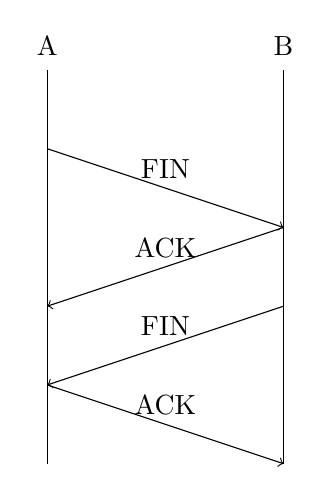
\begin{tikzpicture}
		\draw (-1.5,0) -- (-1.5,-5) (1.5,0) -- (1.5,-5);
		\node at (-1.5,.3) {A};
		\node at (1.5,.3) {B};
		\draw[->] (-1.5,-1) -- node[midway,above] {FIN} (1.5,-2);
		\draw[<-] (-1.5,-3) -- node[midway,above] {ACK} (1.5,-2);
		\draw[<-] (-1.5,-4) -- node[midway,above] {FIN} (1.5,-3);
		\draw[->] (-1.5,-4) -- node[midway,above] {ACK} (1.5,-5);
		\end{tikzpicture}	
		}
	\end{minipage}
	\hfill
	\begin{minipage}[h]{0.3\linewidth}
		\center {
			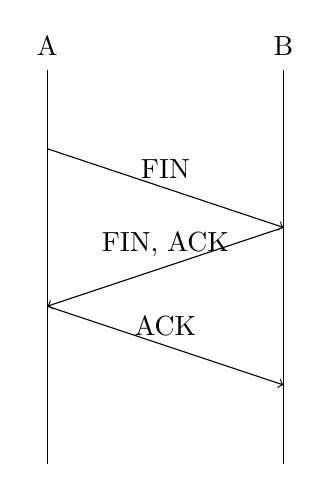
\begin{tikzpicture}
			\draw (-1.5,0) -- (-1.5,-5) (1.5,0) -- (1.5,-5);
			\node at (-1.5,.3) {A};
			\node at (1.5,.3) {B};
			\draw[->] (-1.5,-1) -- node[midway,above] {FIN} (1.5,-2);
			\draw[<-] (-1.5,-3) -- node[midway,above] {FIN, ACK} (1.5,-2);
			\draw[->] (-1.5,-3) -- node[midway,above] {ACK} (1.5,-4);
			\end{tikzpicture}	
		}
	\end{minipage}
	\hfill
	\begin{minipage}[h]{0.3\linewidth}
		\center {
			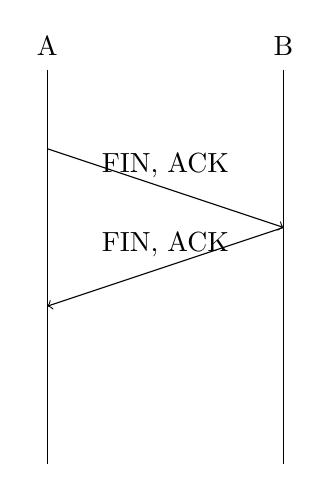
\begin{tikzpicture}
			\draw (-1.5,0) -- (-1.5,-5) (1.5,0) -- (1.5,-5);
			\node at (-1.5,.3) {A};
			\node at (1.5,.3) {B};
			\draw[->] (-1.5,-1) -- node[midway,above] {FIN, ACK} (1.5,-2);
			\draw[<-] (-1.5,-3) -- node[midway,above] {FIN, ACK} (1.5,-2);
			\end{tikzpicture}	
		}
	\end{minipage}
	\vfill
	\caption{Различные варианты завершения соединения}
	\label{fig:tcp_fin}
\end{figure}

Завершение соединения допускает вариативность (см. рис.~\ref{fig:tcp_fin}).
\subsection{Дополнительные флаги}
\begin{itemize}
	\item PSH -- флаг выставляется, когда нужно уведомить получателя о том, чтобы не буферизовывать данные;
	\item URG -- флаг важности, если он поднят, то принимающая сторона должна учитывать поле Urgent pointer (какие данные нужно срочно обработать);
	\item в Reserved используется 2 флага, связанных с перегрузкой сети.
\end{itemize}

\subsection{Опции}
За размер поля Options отвечает поле Header Length. Размер опций всегда кратен 4, если это не так, то вставляются дополнительные NOP байты. 
Некоторые опции:
\begin{itemize}
	\item MSS (Maximum Segment Size) -- максимальный размер сегмента, необходим для роутеров, которые могут менять значение этого поля, основываясь на MTU, для избежания фрагментации; 
	\item SACK/NACK -- позволяет оптимизировать процесс подтверждения, т.е. перечислить в явном виде, какие сегменты были получены, а какие нет;
	\item Scale factor. Максимальный Window Size -- 65 КБ, что не очень эффективно для современных 100 Gb интерфейсов. Поле Scale factor указывает, во сколько раз надо увеличить окно;
\end{itemize}

SCAK/NACK должны поддерживаться с двух сторон, а также на промежуточных устройствах (например, файрволах).

\subsection{Оптимизации}
\begin{itemize}
	\item Fast retransmission;
	\item алгоритм Нейгла;
	\item задержанное подтверждение.
\end{itemize}

\subsection{Некоторые приложения}
\begin{itemize}
	\item FTP;
	\item Telnet;
	\item SMTP.
\end{itemize}

\subsection{Литература}
\begin{itemize}
	\item ICND1 \cite{icnd1eng}, Глава 5;
	\item Олифер \cite{olipher}, Глава 17, с. 554-570.
\end{itemize}